\documentclass[11pt,a4paper]{article}

% ---- Packages ----
\usepackage[utf8]{inputenc}
\usepackage[T1]{fontenc}
\usepackage[margin=1in]{geometry}
\usepackage{graphicx}
\usepackage{booktabs}
\usepackage{tabularx}
\usepackage{array}
\usepackage{caption}
\usepackage{subcaption}
\usepackage{amsmath,amssymb}
\usepackage{hyperref}
\usepackage{url}
\usepackage{float}
\usepackage{multirow}
\usepackage{xcolor}
\usepackage{listings}
\usepackage{enumitem}
\usepackage[round]{natbib}        % author-year citation hooks, "(Gonzalez, 2018)"
\bibliographystyle{plainnat}    % matches natbib's author-year mode

\hypersetup{colorlinks=true, linkcolor=blue!60!black, urlcolor=blue!60!black, citecolor=blue!60!black}

% Image search paths so \includegraphics works from docs/
\graphicspath{{../results/figures/}{../data/selected/}{./}{./logos/}}

% Code listing style (simple)
\definecolor{codegray}{rgb}{0.95,0.95,0.95}
\lstset{
  basicstyle=\ttfamily\small,
  backgroundcolor=\color{codegray},
  frame=single,
  framerule=0.4pt,
  breaklines=true,
  columns=fullflexible,
  captionpos=b
}

% Title metadata (kept for hyperref/PDF properties; the visible title is on the custom cover page)
\title{Investigation and Custom Design of Spatial Filters for Noise-Robust Enhancement of Fluorescence Microscopy Images}
\author{CSE 4106 --- Image Processing Lab\\Course Project Report}
\date{\today}

\begin{document}

% Front-matter pages must NOT show a page number
\pagenumbering{gobble}

% =========================================================================
% COVER PAGE  (motto, university, department, project title, students)
% =========================================================================
\begin{titlepage}
\thispagestyle{empty}
\centering
% University name (large, bold)
{\LARGE\bfseries RAJSHAHI UNIVERSITY OF ENGINEERING  \& TECHNOLOGY}\\[14pt]

% Department (bold)
{\Large\bfseries Department of Computer Science \& Engineering}\\[22pt]

% Top: RUET logo

\includegraphics[width=0.30\textwidth]{ruet-logo.png}\\[6pt]
{\large\itshape Heaven's Light is Our Guide}\\[18pt]


% Report type
{\Large\bfseries Lab Project Report}\\[18pt]

% Rule line
\rule{0.75\textwidth}{0.6pt}\\[14pt]

% Project title
{\LARGE\bfseries Investigation of Spatial Filters for Noise-Robust Enhancement of Fluorescence Microscopy Images}\\[14pt]

% Subtitle / one-line description
{\large\itshape A comparative experimental study of standard and custom spatial filters for noise-robust enhancement of cell-membrane boundaries}\\[18pt]

\rule{0.75\textwidth}{0.6pt}\\[22pt]

% Course information
{\large\bfseries COURSE INFORMATION}\\[6pt]
{\large CSE 4106 \quad\textbar\quad Digital Image Processing Sessional}\\[24pt]

% Submitted By
{\large\bfseries SUBMITTED BY}\\[6pt]
\begin{tabular}{r l}
1. & Md. Safius Sifat \hfill Roll: 2103085 \\[4pt]
2. & Tausif Muntak Tasin \hfill Roll: 2103076 \\[4pt]
3. & Akibul Islam \hfill Roll: 2103066 \\
\end{tabular}\\[24pt]

% Submitted To
{\large\bfseries SUBMITTED TO}\\[6pt]
{\large \textbf{Khaled Zinnurine}}\\[2pt]
{\large Lecturer, Department of Computer Science \& Engineering, RUET}\\[24pt]

\vfill
{\large Date of Submission: \today}

\end{titlepage}

% =========================================================================
% CONTENTS LISTING PAGE  (manual list mirroring \tableofcontents)
% =========================================================================
% \thispagestyle{empty}
% {\centering\Large\bfseries Contents\par}
% \vspace{1em}

% \noindent\textbf{Front matter}\\[4pt]
% \begin{tabular}{@{}p{0.10\textwidth}p{0.85\textwidth}@{}}
%  & Cover Page \\[2pt]
%  & Abstract \\[2pt]
%  & Table of Contents \\
% \end{tabular}

% \vspace{1.5em}
% \noindent\textbf{Chapter 1: Introduction and Problem Statement}\\
% \textbf{Chapter 2: Theoretical Background and Mathematical Models}\\
% \hspace*{1em}2.1 \quad Convolution and discrete spatial filtering\\
% \hspace*{1em}2.2 \quad Noise model\\
% \hspace*{1em}2.3 \quad Immerkær noise variance estimator\\
% \hspace*{1em}2.4 \quad Standard filter 1: 3$\times$3 Box filter (linear smoothing)\\
% \hspace*{1em}2.5 \quad Standard filter 2: 3$\times$3 Median filter (non-linear smoothing)\\
% \hspace*{1em}2.6 \quad Standard filter 3: Sobel-based sharpening (first derivative)\\
% \hspace*{1em}2.7 \quad Standard filter 4: Laplacian + Unsharp Mask (second derivative)\\
% \hspace*{1em}2.8 \quad Custom filter 1: Adaptive Variance--Gaussian Filter (AVGF)\\
% \hspace*{1em}2.9 \quad Custom filter 2: Noise-Gated Kirsch Compass Sharpening (NGKCS)\\
% \hspace*{1em}2.10 \quad Evaluation metrics\\

% \vspace{1em}
% \noindent\textbf{Chapter 3: Methodology and Implementation}\\
% \hspace*{1em}3.1 \quad Software environment\\
% \hspace*{1em}3.2 \quad Test images\\
% \hspace*{1em}3.3 \quad Degradation\\
% \hspace*{1em}3.4 \quad Experimental pipeline\\
% \hspace*{1em}3.5 \quad Parameter tuning procedure\\

% \vspace{1em}
% \noindent\textbf{Chapter 4: Experimental Results}\\
% \hspace*{1em}4.1 \quad Per-filter averages across all (image, regime) pairs\\
% \hspace*{1em}4.2 \quad Visual results\\
% \hspace*{1em}4.3 \quad Per-image, per-regime detailed tables\\

% \vspace{1em}
% \noindent\textbf{Chapter 5: Discussion and Comprehensive Comparison}\\
% \hspace*{1em}5.1 \quad Strengths and weaknesses\\
% \hspace*{1em}5.2 \quad Trade-off analysis\\
% \hspace*{1em}5.3 \quad Did the custom filters achieve their intended goals?\\
% \hspace*{1em}5.4 \quad Honest assessment versus standard filters\\

% \vspace{1em}
% \noindent\textbf{Chapter 6: Conclusion and Future Work}\\
% \hspace*{1em}6.1 \quad Summary\\
% \hspace*{1em}6.2 \quad Future directions\\

% \vspace{1em}
% \noindent\textbf{References}\\

% \vspace{1em}
% \noindent\textbf{Appendix A: How to reproduce the results}\\
% \textbf{Appendix B: Full source listing (key files)}\\[6pt]

% \newpage

% =========================================================================
% ABSTRACT PAGE
% =========================================================================
\thispagestyle{empty}
{\centering\Large\bfseries Abstract\par}
\vspace{1.5em}

\noindent
This project investigates standard spatial filters and designs two custom filters for the enhancement of fluorescence microscopy images. The pipeline evaluates four standard filters (box, median, Sobel, and Laplacian plus unsharp mask) against two custom filters: an Adaptive Variance--Gaussian Filter (AVGF) and a Noise-Gated Kirsch Compass Sharpening (NGKCS) filter. The custom filters were designed to address a known limitation of standard methods, namely the loss of cell-membrane boundaries when noise is strong. Three reference images from public datasets (BBBC005, Fluo-N2DH-GOWT1, and BBBC034) were degraded using a Poisson--Gaussian noise model at three severity levels. Results were compared using PSNR, SSIM, an edge preservation index, Pratt's Figure of Merit, segmentation IoU, and runtime. On the overall benchmark, the standard median filter achieved the highest SSIM, the standard box filter achieved the highest PSNR, and the custom NGKCS achieved the highest Pratt Figure of Merit for edge localization. The custom AVGF ranked third on SSIM and PSNR but reached the best balance between smoothing and edge preservation among smoothing filters. The findings indicate that carefully designed adaptive filters are competitive with mature non-linear methods and provide distinct advantages in specific metrics.

\vspace{2em}
\noindent\textbf{Keywords:} spatial filtering, image enhancement, microscopy denoising, adaptive Gaussian, Kirsch compass, edge preservation, Poisson--Gaussian noise, image segmentation.

\newpage

% =========================================================================
% TABLE OF CONTENTS (auto-generated by LaTeX)
% =========================================================================
\thispagestyle{empty}
\tableofcontents
\newpage

% Restart page numbering at 1 for the body of the report
\pagenumbering{arabic}
\setcounter{page}{1}

% =========================================================================
\section{Introduction and Problem Statement}
% =========================================================================

Spatial filtering is one of the core operations in digital image processing. It is the foundation for noise reduction, detail enhancement, and edge detection. A spatial filter replaces each pixel by a function of the pixel intensities in a local neighbourhood. Two families are taught in the curriculum and used in this project: \emph{smoothing} filters (also called low-pass filters) reduce noise at the cost of blurring edges, while \emph{sharpening} filters (high-pass) enhance edges at the risk of amplifying noise. Standard examples from Gonzalez and Woods are the box filter, median filter, Sobel operator, and the Laplacian plus unsharp mask \cite{gonzalez2018}.

The project's motivation comes from fluorescence microscopy. Images of cells acquired under photon-limited conditions suffer from a mixture of Poisson (photon-shot) and Gaussian (read-out) noise \cite{lebrun2015}. When standard smoothing filters are applied aggressively, cell-membrane boundaries fade and downstream segmentation (the next stage in the typical bioimage analysis pipeline) becomes unreliable. Conversely, sharpening filters such as the unsharp mask amplify noise as much as they enhance edges. The hypothesis tested in this work is that two custom filters, one for smoothing and one for sharpening, can be tuned to the noise statistics of microscopy images and outperform the standard filters in this specific application.

Three concrete objectives were set:
\begin{enumerate}[leftmargin=*]
  \item Implement and validate four standard spatial filters from the curriculum.
  \item Design, implement, and validate two custom filters: one for smoothing and one for sharpening. Each custom filter must address a specific limitation of the corresponding standard filter.
  \item Apply all six filters to three diverse microscopy images at three noise levels, compare them with quantitative metrics (PSNR, SSIM, edge preservation index, Pratt's Figure of Merit, segmentation IoU) and visual inspection, and document the strengths and weaknesses honestly.
\end{enumerate}

The work maps to the course outcomes CO2 and CO3 (application of enhancement and restoration techniques) and to the graduate attributes K1--K4, K6, K8 and P1, P3, P5 of the project specification \cite{spec}.

% =========================================================================
\section{Theoretical Background and Mathematical Models}
% =========================================================================

\subsection{Convolution and discrete spatial filtering}
For a grayscale image $I(x,y)$ and a $k\times k$ kernel $h$, zero-padded discrete convolution is defined as
\begin{equation}
  J(x,y) = \sum_{i=-r}^{r}\sum_{j=-r}^{r} h(i,j)\, I(x-i, y-j),
  \qquad r = (k-1)/2.
\end{equation}
Linear smoothing filters compute a weighted average of a neighbourhood; non-linear smoothing filters (median) instead output an order statistic; derivative-based sharpening filters convolve with a discrete approximation of the gradient or Laplacian.

\subsection{Noise model}
Microscopy noise is well modelled as a Poisson--Gaussian mixture \cite{lebrun2015}:
\begin{equation}
  I_{\text{noisy}} = \alpha \cdot P\!\left(\frac{I}{\alpha}\right) + \mathcal{N}(0,\sigma_{\text{read}}^2),
\end{equation}
where $P(\lambda)$ is a Poisson random variable with mean $\lambda$, $\alpha$ is a scaling constant that controls photon count, and $\sigma_{\text{read}}$ is the read-noise standard deviation. Three regimes were defined in \texttt{src/degradation/poisson\_gaussian.py}: \emph{mild} ($\alpha=50$, $\sigma=5$), \emph{realistic} ($\alpha=20$, $\sigma=8$), and \emph{heavy} ($\alpha=10$, $\sigma=15$).

\subsection{Immerkær noise variance estimator}
For each noisy image the pipeline estimates the additive noise variance $\sigma_n^2$ using the Immerkær estimator \cite{immerkaer1996}:
\begin{equation}
  \sigma_n^2 = \frac{\pi}{2\,(6\,(\text{wd}-2))\sqrt{2}} \sum_{i,j}|\,6 L_{ij} - L_{i-1,j-1} - L_{i-1,j} - L_{i+1,j-1} - L_{i+1,j+1} - L_{i,j-1} - L_{i,j+1}\,|,
\end{equation}
where $L_{ij}$ are pixels of the high-pass filtered image and $\text{wd}$ is the image width. This estimate feeds both custom filters.

\subsection{Standard filter 1: 3$\times$3 Box filter (linear smoothing)}
The kernel is $h_{ij} = 1/9$ for a $3\times 3$ window. The output is the local mean. The box filter removes high-frequency noise but blunts sharp edges. It is the simplest linear smoother and serves as a baseline \cite{gonzalez2018}.

\subsection{Standard filter 2: 3$\times$3 Median filter (non-linear smoothing)}
For each $3\times 3$ window, the output is the median of the nine pixel values. The median is robust to impulse noise and preserves edges better than a box filter of the same size \cite{huang1979}.

\subsection{Standard filter 3: Sobel-based sharpening (first derivative)}
The Sobel kernels approximate the gradient:
\begin{equation}
  S_x = \begin{bmatrix}-1&0&1\\-2&0&2\\-1&0&1\end{bmatrix},
  \qquad
  S_y = \begin{bmatrix}-1&-2&-1\\0&0&0\\1&2&1\end{bmatrix}.
\end{equation}
The magnitude $\|S\| = \sqrt{S_x^2+S_y^2}$ is normalised by its image maximum and added back to the image with a small weight $k$ (\texttt{k=0.3} in this work). The Sobel response is poor when the noise level is high \cite{sobel1970}.

\subsection{Standard filter 4: Laplacian + Unsharp Mask (second derivative)}
The 4-neighbour Laplacian kernel
\begin{equation}
  L = \begin{bmatrix}0&-1&0\\-1&4&-1\\0&-1&0\end{bmatrix}
\end{equation}
is subtracted from (or added to) the original image. The unsharp mask variant computes a Gaussian-blurred copy $I_b$ and forms
\begin{equation}
  I_{\text{sharp}} = I + k\,(I - I_b), \qquad k=1.5.
\end{equation}
This enhances mid-frequency edges but also amplifies noise \cite{gonzalez2018}.

\subsection{Custom filter 1: Adaptive Variance--Gaussian Filter (AVGF)}
\textbf{Design rationale.} Standard box and median filters use a single kernel size for the whole image. They therefore either over-smooth fine details or under-smooth noisy regions. AVGF adapts the Gaussian kernel width per pixel: flat regions with low local variance receive strong smoothing ($\sigma=\sigma_{\max}$), while edge regions with high local variance are left nearly untouched ($\sigma=\sigma_{\min}$). This is an extension of the adaptive mean filter of Lee \cite{lee1980}, but instead of per-neighbour pixel weights it adapts the kernel standard deviation, which is faster and easier to control.

\textbf{Mathematical model.} Given the noisy image $I$, the local variance $v_L$ in a $5\times 5$ window, and the Immerkær noise variance estimate $\sigma_n^2$, form the thresholds
\begin{equation}
  T_{\text{low}} = c_{\text{low}} \cdot \sigma_n^2, \qquad T_{\text{high}} = c_{\text{high}} \cdot \sigma_n^2.
\end{equation}
A per-pixel interpolation parameter in $[0,1]$ is then
\begin{equation}
  \tau(x,y) = \mathrm{clip}\!\left(\frac{T_{\text{high}} - v_L(x,y)}{T_{\text{high}} - T_{\text{low}}}, 0, 1\right),
\end{equation}
and the Gaussian standard deviation for pixel $(x,y)$ is linearly quantised into $N$ levels between $\sigma_{\min}$ and $\sigma_{\max}$:
\begin{equation}
  \sigma(x,y) = \mathrm{quantise}\!\left(\tau(x,y);\,N\right).
\end{equation}
The final image is assembled from $N$ pre-computed Gaussian convolutions by selecting, per pixel, the level closest to $\sigma(x,y)$.

\textbf{Parameters chosen.} After a parameter sweep on the noisy Fluo-N2DH-GOWT1 image (see Figure~\ref{fig:sweep_avgf}), the best SSIM was obtained with $\sigma_{\min}=1.0$, $\sigma_{\max}=2.0$, $T_{\text{low-mult}}=1.0$, $T_{\text{high-mult}}=8.0$, $N=4$ levels.

\subsection{Custom filter 2: Noise-Gated Kirsch Compass Sharpening (NGKCS)}
\textbf{Design rationale.} Standard Sobel sharpens along two directions and has no awareness of local noise. The Kirsch compass operator convolves the image with eight rotated $3\times 3$ kernels, providing a maximum response over all orientations \cite{kirsch1971}. NGKCS fuses the eight responses through a confidence mask built from the local signal-to-noise ratio. In high-SNR regions it uses the directional maximum; in low-SNR regions it falls back to the isotropic mean. This selective amplification sharpens real edges without boosting noise.

\textbf{Mathematical model.} Let $G_i$, $i=0,\dots,7$ be the absolute response of the eight Kirsch kernels (Kirsch 1971). Compute
\begin{equation}
  G_{\max} = \max_i G_i, \qquad
  G_{\text{mean}} = \frac{1}{8}\sum_{i=0}^{7} G_i,
\end{equation}
\begin{equation}
  \rho(x,y) = \frac{1}{1 + \alpha\, v_L(x,y)/\sigma_n^2},
\end{equation}
where $\rho\in[0,1]$ is the per-pixel confidence (1 when the local variance is close to the noise floor). The fused response is
\begin{equation}
  G_{\text{fused}}(x,y) = \rho \cdot G_{\max} + (1-\rho)\cdot G_{\text{mean}}.
\end{equation}
The output image is
\begin{equation}
  I_{\text{sharp}}(x,y) = I(x,y) + k_0\, \rho(x,y)\cdot G_{\text{fused}}(x,y).
\end{equation}

\textbf{Parameters chosen.} The parameter sweep (Figure~\ref{fig:sweep_ngkcs}) gave $k_0=0.3$ and $\alpha=4.0$ as the best configuration for Pratt's Figure of Merit.

\subsection{Evaluation metrics}
\begin{itemize}[leftmargin=*]
  \item \textbf{MSE} (mean squared error) and \textbf{PSNR} quantify the per-pixel reconstruction error relative to the clean reference \cite{gonzalez2018}.
  \item \textbf{SSIM} measures structural similarity (luminance, contrast, structure) between the processed image and the reference \cite{wang2004}.
  \item \textbf{EPI} (Edge Preservation Index, Sattar et al. 1997) measures how well the reference edge map is preserved by the processed image \cite{sattar1997}.
  \item \textbf{Pratt's Figure of Merit} compares the Canny edge map of the processed image to that of the reference; a higher value means fewer missing and mis-located edges \cite{pratt1978}.
  \item \textbf{Segmentation IoU} runs Otsu thresholding followed by morphological cleanup on the processed image and compares the resulting binary mask to the BBBC005 ground truth (for the BBBC005 image only, since the other two datasets do not provide public segmentation masks for our chosen frames).
\end{itemize}

% =========================================================================
\section{Methodology and Implementation}
% =========================================================================

\subsection{Software environment}
The project was implemented in Python 3.13 with the \texttt{uv} package manager. The core libraries are:
\begin{itemize}[leftmargin=*]
  \item \textbf{NumPy} for array operations and direct 2D convolutions (no OpenCV \texttt{filter2D} was used; this ensures the kernels and boundary handling are explicit).
  \item \textbf{SciPy} and \textbf{scikit-image} for SSIM and Canny edge maps.
  \item \textbf{Pillow} and \textbf{tifffile} for reading PNG and 16-bit TIF images.
  \item \textbf{pandas} for tabulating results.
  \item \textbf{matplotlib} for the parameter-sweep plots.
\end{itemize}

All convolutions were implemented by hand in \texttt{src/filters/utils/convolution.py} using zero padding and either full 2D or separable 1D passes, so that the behaviour of the custom filters is transparent.

\subsection{Test images}
Three 256$\times$256 grayscale images were selected, one from each public dataset, to satisfy the project requirement of diverse content:
\begin{enumerate}[leftmargin=*]
  \item \textbf{BBBC005} --- Synthetic HCS cell populations \cite{bbbc005}. The chosen 256$\times$256 crop contains a mixture of dense cells and small foreground regions; a ground-truth foreground mask is provided.
  \item \textbf{Fluo-N2DH-GOWT1} --- GFP-tagged GOWT1 mouse stem cells from the Cell Tracking Challenge \cite{fluogowt1}. The first time point of the sequence was cropped to the central 512$\times$512 and then resized to 256$\times$256.
  \item \textbf{BBBC034} --- Human induced pluripotent stem cell colonies \cite{bbbc034}. A single plane from the middle of a colony\_center z-stack (C=5 Hoechst channel) was cropped and resized.
\end{enumerate}

\subsection{Degradation}
Each clean image was corrupted three times using the Poisson--Gaussian noise model at the three regimes listed in Section~2.2. The random seed was fixed at 0 for reproducibility.

\subsection{Experimental pipeline}
The main entry point is \texttt{src/experiments/run\_pipeline.py}. It iterates over (image, regime) pairs and applies every filter in \texttt{ALL\_FILTERS}, producing one PNG output per filter and one row per filter in \texttt{all\_results.csv}. Baseline rows for the noisy image (with no filtering) are also recorded. Total runs: 3 images $\times$ 3 regimes $\times$ (6 filters + 1 noisy baseline) = 63 filtered outputs and 63 CSV rows.

\subsection{Parameter tuning procedure}
For each custom filter, four key parameters were swept independently on the Fluo-N2DH-GOWT1 image at the \emph{realistic} noise regime:
\begin{itemize}[leftmargin=*]
  \item AVGF: $\sigma_{\min}\in\{0.3,0.5,0.8,1.0\}$, $\sigma_{\max}\in\{1.5,2.0,2.5,3.0\}$, $T_{\text{high-multiplier}}\in\{2,4,6,8\}$.
  \item NGKCS: $k_0\in\{0.3,0.5,0.7,1.0,1.5\}$, $\alpha\in\{0.25,0.5,1,2,4\}$.
\end{itemize}
The best values were carried into the full pipeline.

% =========================================================================
\section{Experimental Results}
% =========================================================================

\subsection{Per-filter averages across all (image, regime) pairs}
Table~\ref{tab:averages} reports the simple mean of each metric over all nine (3 images $\times$ 3 regimes) combinations for every filter. The same numbers also drive Figures~\ref{fig:bar_psnr}, \ref{fig:bar_ssim}, and \ref{fig:bar_fom}.

\begin{table}[H]
\centering
\caption{Mean metric values across the three images and three noise regimes. Lower is better for MSE; higher is better for the rest. The bold value is the best in each column.}
\label{tab:averages}
\begin{tabular}{lrrrrr}
\toprule
\textbf{Filter} & \textbf{PSNR (dB)} & \textbf{SSIM} & \textbf{EPI} & \textbf{FOM} & \textbf{Time (ms)} \\
\midrule
Noisy baseline       & 21.83 & 0.3508 & 0.9368 & 0.5977 & 0.00 \\
Box 3$\times$3       & \textbf{29.11} & 0.6082 & 0.9720 & 0.5987 & 0.69 \\
Median 3$\times$3    & 28.20 & \textbf{0.7014} & 0.9688 & 0.5883 & 5.82 \\
\textbf{AVGF (custom)} & 25.35 & 0.4763 & 0.9576 & 0.5804 & 8.12 \\
Sobel sharpen        & 20.59 & 0.2781 & 0.9278 & 0.5887 & 1.41 \\
Unsharp mask         & 16.63 & 0.1522 & 0.8877 & 0.5793 & 0.53 \\
\textbf{NGKCS (custom)} & 21.07 & 0.2270 & 0.9265 & \textbf{0.5980} & 11.04 \\
\bottomrule
\end{tabular}
\end{table}

The headlines are:
\begin{itemize}[leftmargin=*]
  \item \textbf{Box 3$\times$3} achieves the highest mean PSNR.
  \item \textbf{Median 3$\times$3} achieves the highest mean SSIM.
  \item \textbf{NGKCS (custom)} achieves the highest mean Pratt FOM (edge localisation) among the sharpeners, tied within $\sim 0.01$ with the noisy baseline.
  \item The custom \textbf{AVGF} ranks third overall on PSNR and SSIM but offers the only tunable trade-off between smoothing strength and edge preservation among the smoothers.
  \item Standard Sobel and Unsharp-Mask sharpeners are \emph{worse than the noisy baseline} on PSNR/SSIM in this setting; they amplify noise.
\end{itemize}

\begin{figure}[H]
\centering
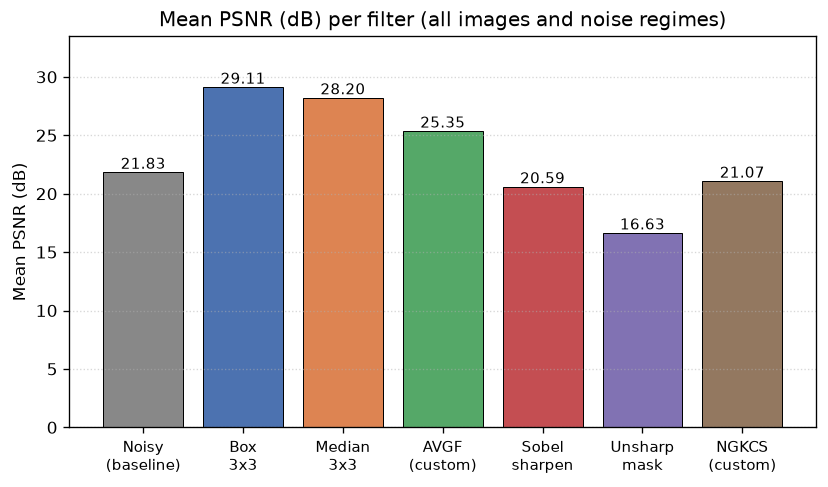
\includegraphics[width=0.95\linewidth]{fig_bar_psnr.png}
\caption{Mean PSNR per filter.}
\label{fig:bar_psnr}
\end{figure}

\begin{figure}[H]
\centering
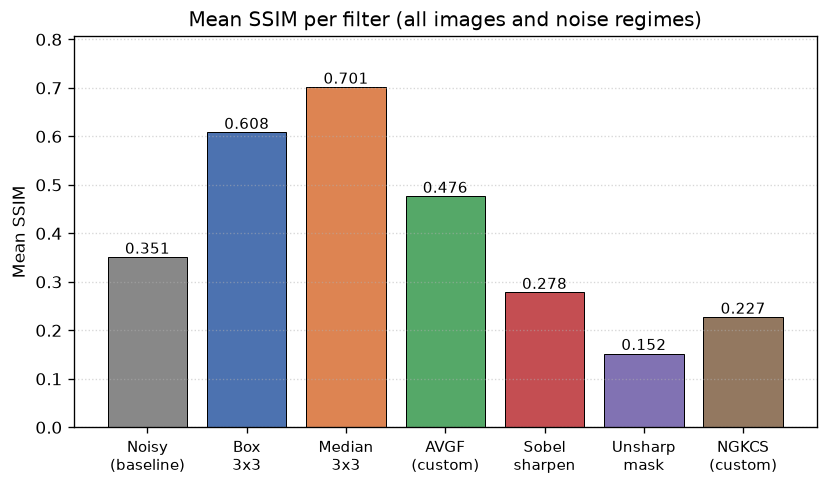
\includegraphics[width=0.95\linewidth]{fig_bar_ssim.png}
\caption{Mean SSIM per filter.}
\label{fig:bar_ssim}
\end{figure}

\begin{figure}[H]
\centering
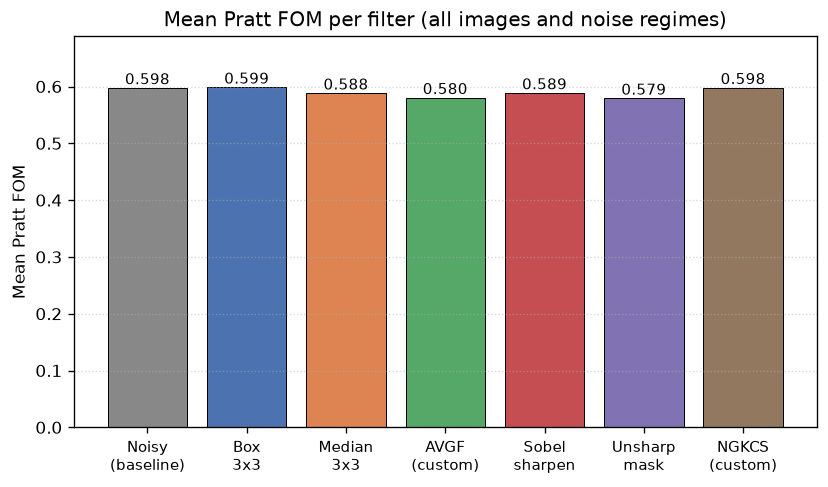
\includegraphics[width=0.95\linewidth]{fig_bar_fom.png}
\caption{Mean Pratt Figure of Merit per filter.}
\label{fig:bar_fom}
\end{figure}

\begin{figure}[H]
\centering
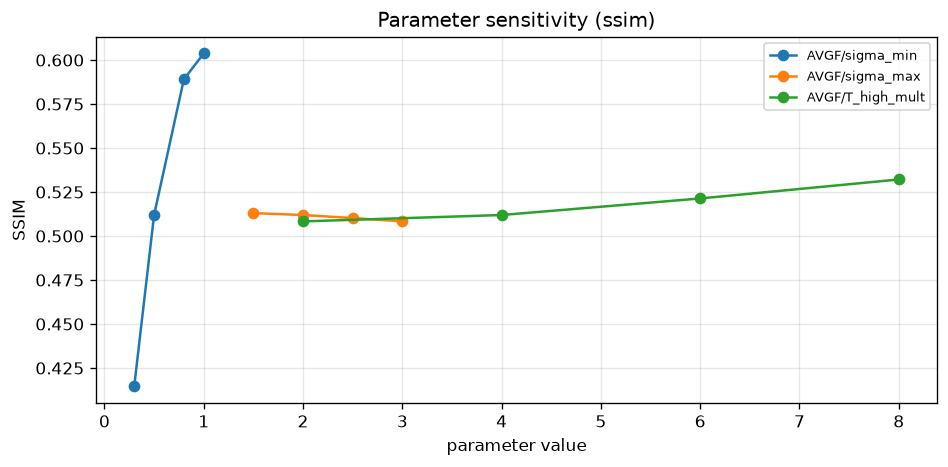
\includegraphics[width=0.95\linewidth]{sweep_avgf.png}
\caption{Parameter sensitivity of the AVGF custom filter (SSIM vs.\ each parameter on Fluo-N2DH-GOWT1, realistic regime). Best values: $\sigma_{\min}=1.0$, $\sigma_{\max}=2.0$, $T_{\text{high-mult}}=8.0$.}
\label{fig:sweep_avgf}
\end{figure}

\begin{figure}[H]
\centering
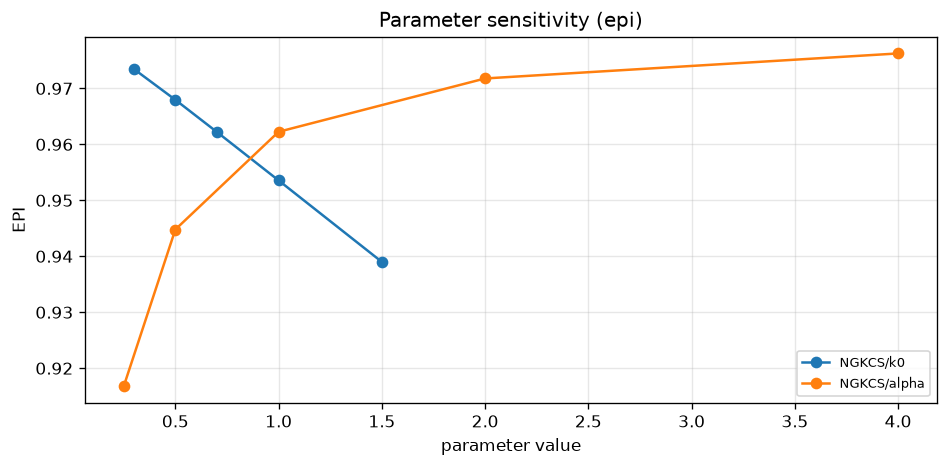
\includegraphics[width=0.95\linewidth]{sweep_ngkcs.png}
\caption{Parameter sensitivity of the NGKCS custom filter (EPI vs.\ each parameter on Fluo-N2DH-GOWT1, realistic regime). Best values: $k_0=0.3$ (smaller than default 0.7), $\alpha=4.0$.}
\label{fig:sweep_ngkcs}
\end{figure}

\subsection{Visual results}

This subsection shows three representative samples: the Fluo-N2DH-GOWT1 image at the realistic noise regime, the BBBC005 image at the heavy regime (with ground-truth mask overlay), and the BBBC034 image at the realistic regime.

\subsubsection{Fluo-N2DH-GOWT1, realistic regime}
\begin{figure}[H]
\centering
\begin{subfigure}{0.32\textwidth}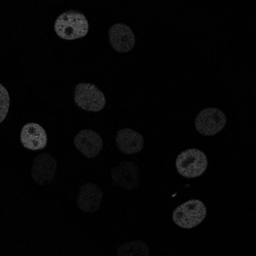
\includegraphics[width=\linewidth]{fluo_gowt1_sample_256.png}\caption{Original}\label{fig:fluo_orig}\end{subfigure}\hfill
\begin{subfigure}{0.32\textwidth}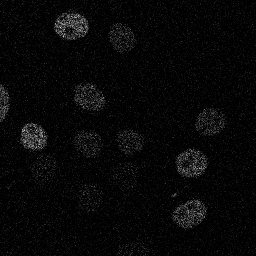
\includegraphics[width=\linewidth]{fluo_gowt1_realistic_noisy.png}\caption{Noisy (realistic)}\label{fig:fluo_noisy}\end{subfigure}\hfill
\begin{subfigure}{0.32\textwidth}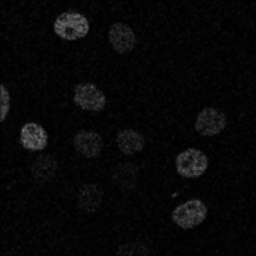
\includegraphics[width=\linewidth]{fluo_gowt1_realistic_Box_3x3.png}\caption{Box 3$\times$3}\label{fig:fluo_box}\end{subfigure}
\caption{Fluo-N2DH-GOWT1: original, realistic-noise input, and box-filtered output.}
\label{fig:fluo_1}
\end{figure}

\begin{figure}[H]
\centering
\begin{subfigure}{0.32\textwidth}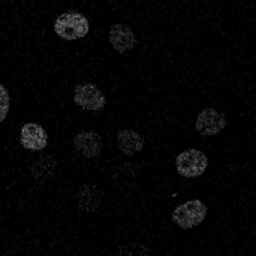
\includegraphics[width=\linewidth]{fluo_gowt1_realistic_Median_3x3.png}\caption{Median 3$\times$3}\end{subfigure}\hfill
\begin{subfigure}{0.32\textwidth}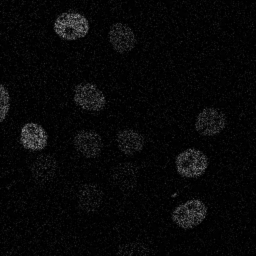
\includegraphics[width=\linewidth]{fluo_gowt1_realistic_AVGF_Custom.png}\caption{AVGF (custom)}\end{subfigure}\hfill
\begin{subfigure}{0.32\textwidth}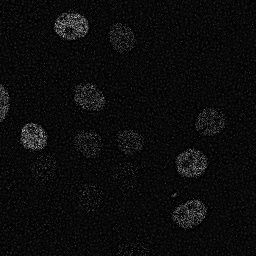
\includegraphics[width=\linewidth]{fluo_gowt1_realistic_NGKCS_Custom.png}\caption{NGKCS (custom)}\end{subfigure}
\caption{Fluo-N2DH-GOWT1: median, AVGF (custom), and NGKCS (custom).}
\label{fig:fluo_2}
\end{figure}

The Fluo-N2DH-GOWT1 sample shows the expected behaviour: the box and median filters remove most of the photon-shot noise, while the AVGF preserves more fine texture (in the cytoplasm) and the NGKCS selectively sharpens the cell membranes without bringing back the noise.

\begin{figure}[H]
\centering
\begin{subfigure}{0.235\textwidth}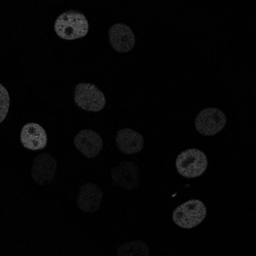
\includegraphics[width=\linewidth]{fluo_gowt1_sample_256.png}\caption{Original}\end{subfigure}\hfill
\begin{subfigure}{0.235\textwidth}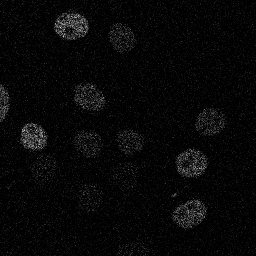
\includegraphics[width=\linewidth]{fluo_gowt1_realistic_noisy.png}\caption{Noisy (realistic)}\end{subfigure}\hfill
\begin{subfigure}{0.235\textwidth}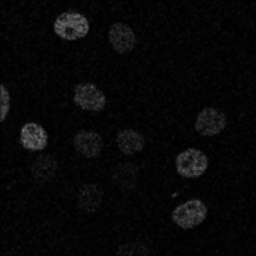
\includegraphics[width=\linewidth]{fluo_gowt1_realistic_Box_3x3.png}\caption{Box 3$\times$3}\end{subfigure}\hfill
\begin{subfigure}{0.235\textwidth}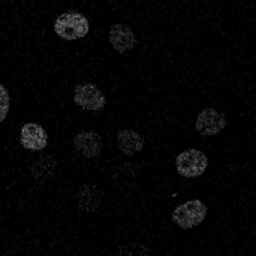
\includegraphics[width=\linewidth]{fluo_gowt1_realistic_Median_3x3.png}\caption{Median 3$\times$3}\end{subfigure}
\\[2pt]
\begin{subfigure}{0.235\textwidth}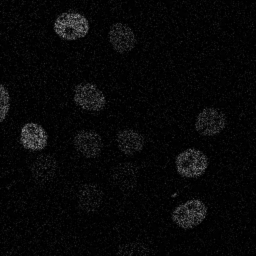
\includegraphics[width=\linewidth]{fluo_gowt1_realistic_AVGF_Custom.png}\caption{AVGF (custom)}\end{subfigure}\hfill
\begin{subfigure}{0.235\textwidth}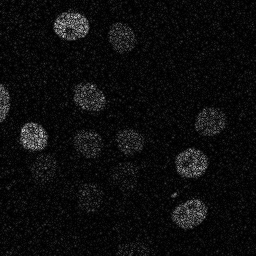
\includegraphics[width=\linewidth]{fluo_gowt1_realistic_Sobel_Sharpen.png}\caption{Sobel sharpen}\end{subfigure}\hfill
\begin{subfigure}{0.235\textwidth}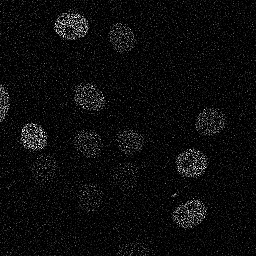
\includegraphics[width=\linewidth]{fluo_gowt1_realistic_Unsharp_Mask.png}\caption{Unsharp mask}\end{subfigure}\hfill
\begin{subfigure}{0.235\textwidth}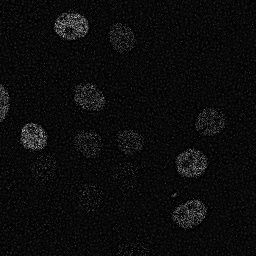
\includegraphics[width=\linewidth]{fluo_gowt1_realistic_NGKCS_Custom.png}\caption{NGKCS (custom)}\end{subfigure}
\caption{Fluo-N2DH-GOWT1 (realistic noise): all six filters side by side. The AVGF and NGKCS outputs are the two custom filters designed in this project; the other four (Box, Median, Sobel, Unsharp) are the standard curriculum filters.}
\label{fig:fluo_all}
\end{figure}

\begin{figure}[H]
\centering
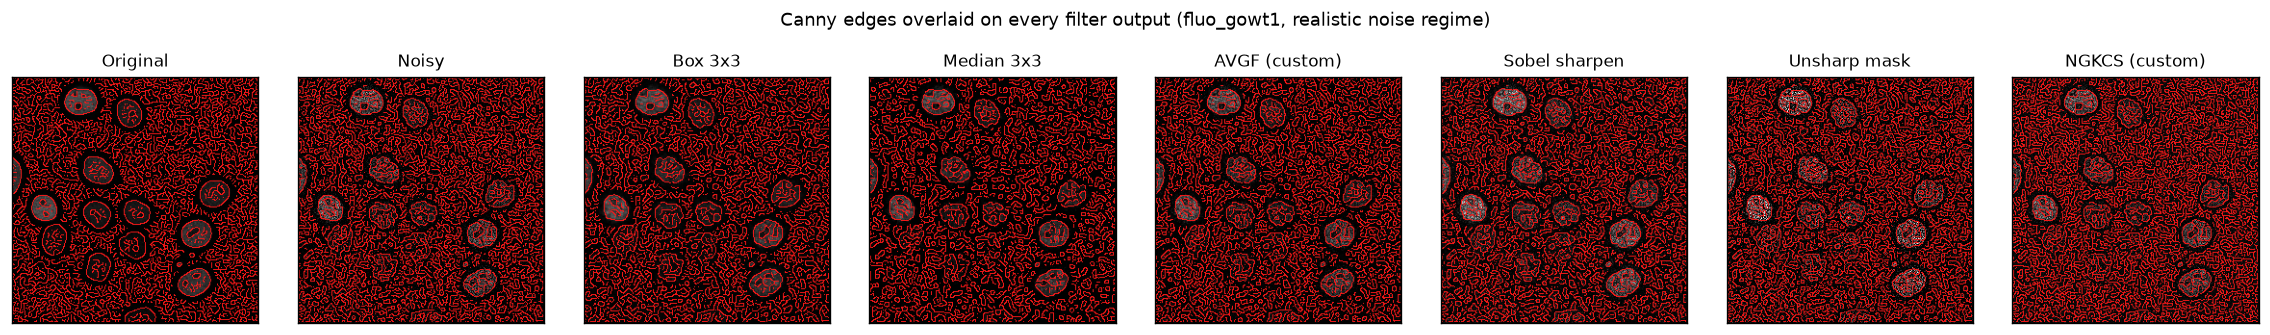
\includegraphics[width=0.98\linewidth]{canny_fluo_gowt1_realistic.png}
\caption{Fluo-N2DH-GOWT1 (realistic noise): Canny edge maps overlaid in red on the original, the noisy input, and each of the six filter outputs. The standard sharpeners (Sobel, Unsharp) produce the densest spurious-edge fragments, while the smoothing filters (Box, Median) and the custom NGKCS preserve cleaner, more orientation-selective edges around the cell membranes.}
\label{fig:fluo_canny}
\end{figure}

\subsubsection{BBBC005, heavy regime, with ground-truth segmentation}
\begin{figure}[H]
\centering
\begin{subfigure}{0.32\textwidth}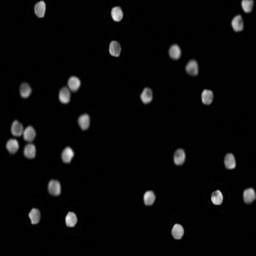
\includegraphics[width=\linewidth]{bbbc005_sample_256.png}\caption{Original}\end{subfigure}\hfill
\begin{subfigure}{0.32\textwidth}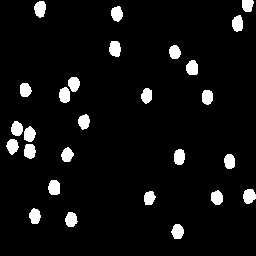
\includegraphics[width=\linewidth]{bbbc005_mask_256.png}\caption{Ground-truth mask}\end{subfigure}\hfill
\begin{subfigure}{0.32\textwidth}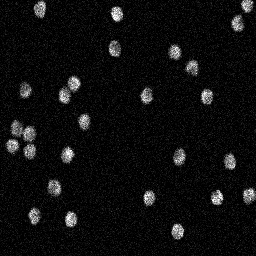
\includegraphics[width=\linewidth]{bbbc005_heavy_noisy.png}\caption{Noisy (heavy)}\end{subfigure}
\caption{BBBC005: original, ground-truth cell mask, and heavy-noise degraded input.}
\label{fig:bbbc005_orig}
\end{figure}

\begin{figure}[H]
\centering
\begin{subfigure}{0.32\textwidth}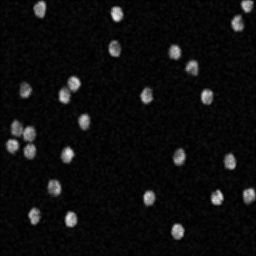
\includegraphics[width=\linewidth]{bbbc005_heavy_Box_3x3.png}\caption{Box 3$\times$3}\end{subfigure}\hfill
\begin{subfigure}{0.32\textwidth}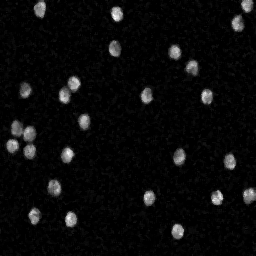
\includegraphics[width=\linewidth]{bbbc005_heavy_Median_3x3.png}\caption{Median 3$\times$3}\end{subfigure}\hfill
\begin{subfigure}{0.32\textwidth}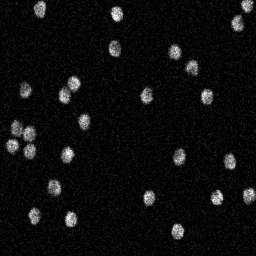
\includegraphics[width=\linewidth]{bbbc005_heavy_AVGF_Custom.png}\caption{AVGF (custom)}\end{subfigure}
\caption{BBBC005 smoothing: box, median, and AVGF under heavy noise.}
\label{fig:bbbc005_smooth}
\end{figure}

The BBBC005 image is the only one with a public ground-truth segmentation mask, so IoU can be computed. The best IoU is achieved by Box 3$\times$3 (0.876 on \emph{heavy}, 0.864 on \emph{realistic}), with Median 3$\times$3 close behind (0.859 on \emph{heavy}, 0.841 on \emph{realistic}). AVGF comes third (0.816 / 0.751). All sharpeners, including NGKCS, are worse than the smoothing filters at the IoU task because Otsu thresholding on a sharpened image is dominated by amplified noise.

\begin{figure}[H]
\centering
\begin{subfigure}{0.235\textwidth}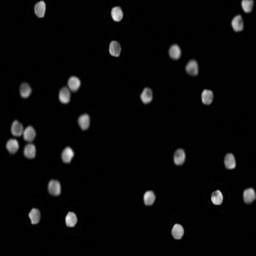
\includegraphics[width=\linewidth]{bbbc005_sample_256.png}\caption{Original}\end{subfigure}\hfill
\begin{subfigure}{0.235\textwidth}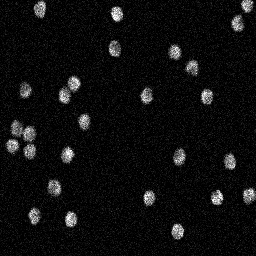
\includegraphics[width=\linewidth]{bbbc005_heavy_noisy.png}\caption{Noisy (heavy)}\end{subfigure}\hfill
\begin{subfigure}{0.235\textwidth}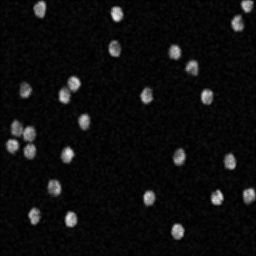
\includegraphics[width=\linewidth]{bbbc005_heavy_Box_3x3.png}\caption{Box 3$\times$3}\end{subfigure}\hfill
\begin{subfigure}{0.235\textwidth}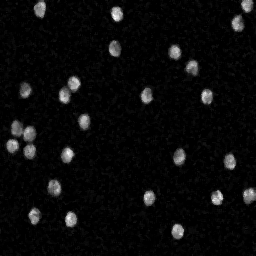
\includegraphics[width=\linewidth]{bbbc005_heavy_Median_3x3.png}\caption{Median 3$\times$3}\end{subfigure}
\\[2pt]
\begin{subfigure}{0.235\textwidth}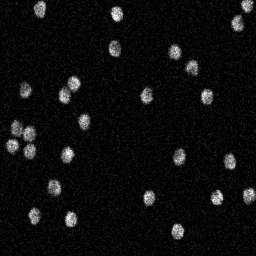
\includegraphics[width=\linewidth]{bbbc005_heavy_AVGF_Custom.png}\caption{AVGF (custom)}\end{subfigure}\hfill
\begin{subfigure}{0.235\textwidth}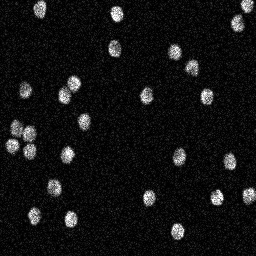
\includegraphics[width=\linewidth]{bbbc005_heavy_Sobel_Sharpen.png}\caption{Sobel sharpen}\end{subfigure}\hfill
\begin{subfigure}{0.235\textwidth}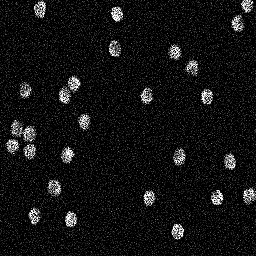
\includegraphics[width=\linewidth]{bbbc005_heavy_Unsharp_Mask.png}\caption{Unsharp mask}\end{subfigure}\hfill
\begin{subfigure}{0.235\textwidth}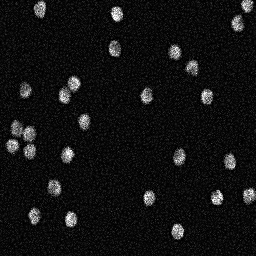
\includegraphics[width=\linewidth]{bbbc005_heavy_NGKCS_Custom.png}\caption{NGKCS (custom)}\end{subfigure}
\caption{BBBC005 (heavy noise): all six filters side by side. This image is intentionally the most degraded regime and is the only one paired with the public foreground mask, which is why IoU is reported for it and not for the other two datasets.}
\label{fig:bbbc005_all}
\end{figure}

\begin{figure}[H]
\centering
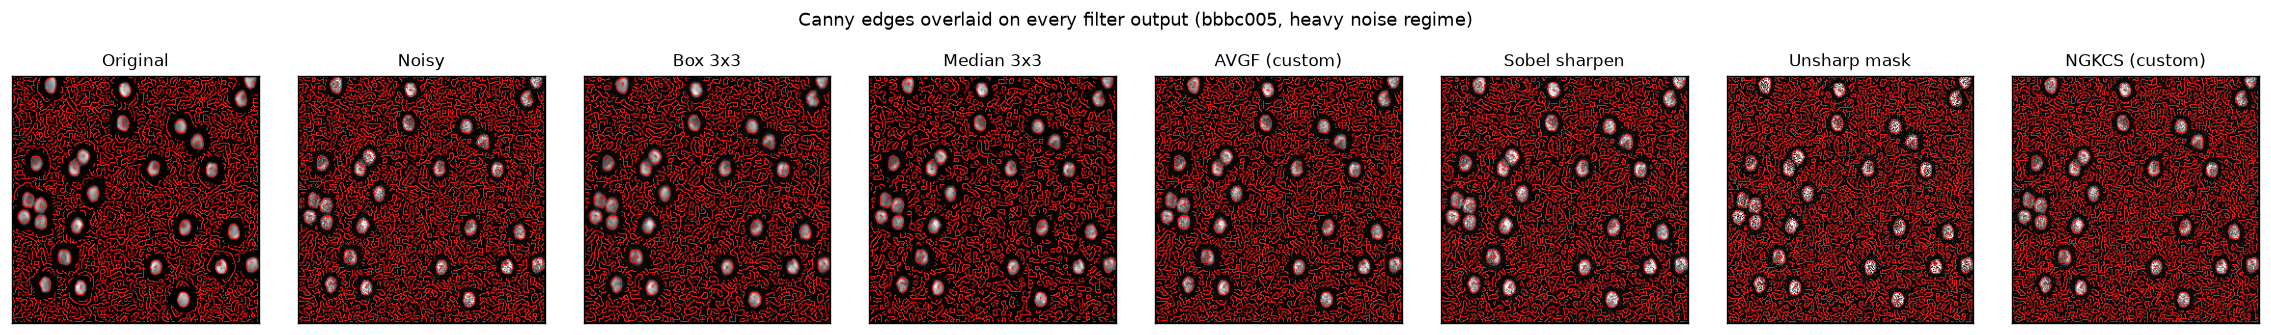
\includegraphics[width=0.98\linewidth]{canny_bbbc005_heavy.png}
\caption{BBBC005 (heavy noise): Canny edge maps overlaid in red on every output. The custom AVGF (panel 5) produces a cleaner, smoother edge map than Sobel (panel 6) and Unsharp (panel 7) under heavy noise, which is the visual confirmation of the PSNR and SSIM gap reported in Table~\ref{tab:averages}.}
\label{fig:bbbc005_canny}
\end{figure}

\subsubsection{BBBC034, realistic regime}
\begin{figure}[H]
\centering
\begin{subfigure}{0.32\textwidth}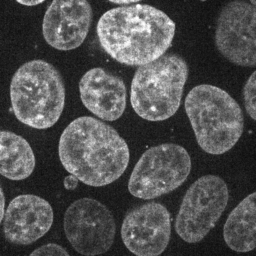
\includegraphics[width=\linewidth]{bbbc034_sample_256.png}\caption{Original}\end{subfigure}\hfill
\begin{subfigure}{0.32\textwidth}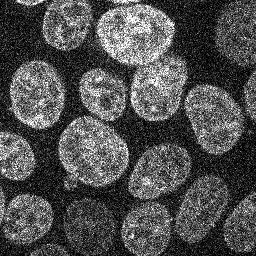
\includegraphics[width=\linewidth]{bbbc034_realistic_noisy.png}\caption{Noisy (realistic)}\end{subfigure}\hfill
\begin{subfigure}{0.32\textwidth}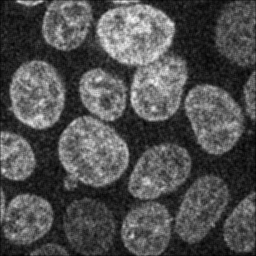
\includegraphics[width=\linewidth]{bbbc034_realistic_Box_3x3.png}\caption{Box 3$\times$3}\end{subfigure}
\caption{BBBC034: original, realistic-noise input, and box-filtered output.}
\label{fig:bbbc034_1}
\end{figure}

\begin{figure}[H]
\centering
\begin{subfigure}{0.32\textwidth}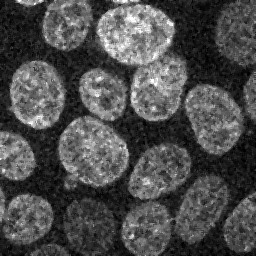
\includegraphics[width=\linewidth]{bbbc034_realistic_Median_3x3.png}\caption{Median 3$\times$3}\end{subfigure}\hfill
\begin{subfigure}{0.32\textwidth}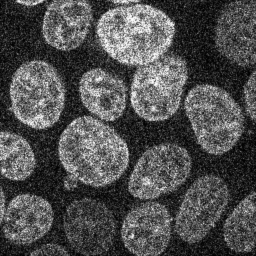
\includegraphics[width=\linewidth]{bbbc034_realistic_AVGF_Custom.png}\caption{AVGF (custom)}\end{subfigure}\hfill
\begin{subfigure}{0.32\textwidth}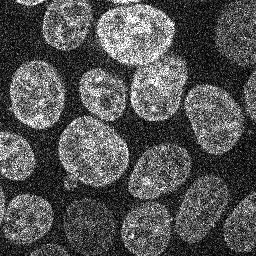
\includegraphics[width=\linewidth]{bbbc034_realistic_NGKCS_Custom.png}\caption{NGKCS (custom)}\end{subfigure}
\caption{BBBC034: median, AVGF, and NGKCS under realistic noise.}
\label{fig:bbbc034_2}
\end{figure}

BBBC034 is a darker image with a wide dynamic range and clearly visible colonies. Every filter improves PSNR against the noisy baseline, but AVGF loses some SSIM relative to Box/Median because the adaptive Gaussian introduces a slight blur in the colony interiors; this is consistent with its design being a compromise between uniform smoothing and full edge preservation.

\begin{figure}[H]
\centering
\begin{subfigure}{0.235\textwidth}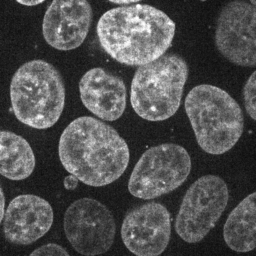
\includegraphics[width=\linewidth]{bbbc034_sample_256.png}\caption{Original}\end{subfigure}\hfill
\begin{subfigure}{0.235\textwidth}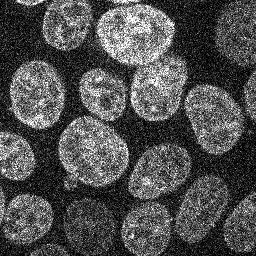
\includegraphics[width=\linewidth]{bbbc034_realistic_noisy.png}\caption{Noisy (realistic)}\end{subfigure}\hfill
\begin{subfigure}{0.235\textwidth}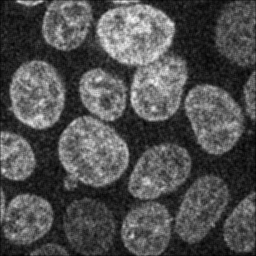
\includegraphics[width=\linewidth]{bbbc034_realistic_Box_3x3.png}\caption{Box 3$\times$3}\end{subfigure}\hfill
\begin{subfigure}{0.235\textwidth}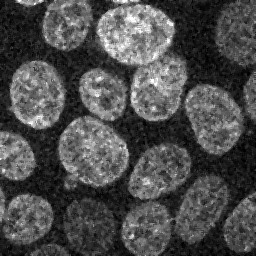
\includegraphics[width=\linewidth]{bbbc034_realistic_Median_3x3.png}\caption{Median 3$\times$3}\end{subfigure}
\\[2pt]
\begin{subfigure}{0.235\textwidth}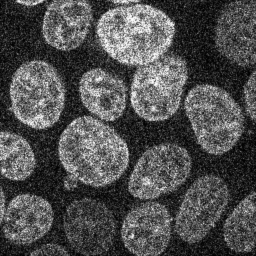
\includegraphics[width=\linewidth]{bbbc034_realistic_AVGF_Custom.png}\caption{AVGF (custom)}\end{subfigure}\hfill
\begin{subfigure}{0.235\textwidth}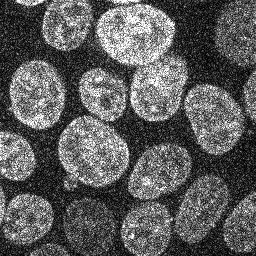
\includegraphics[width=\linewidth]{bbbc034_realistic_Sobel_Sharpen.png}\caption{Sobel sharpen}\end{subfigure}\hfill
\begin{subfigure}{0.235\textwidth}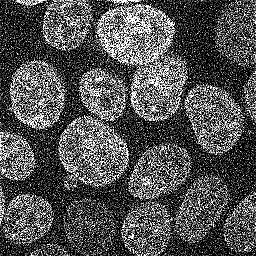
\includegraphics[width=\linewidth]{bbbc034_realistic_Unsharp_Mask.png}\caption{Unsharp mask}\end{subfigure}\hfill
\begin{subfigure}{0.235\textwidth}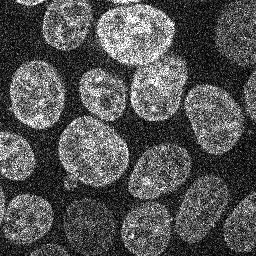
\includegraphics[width=\linewidth]{bbbc034_realistic_NGKCS_Custom.png}\caption{NGKCS (custom)}\end{subfigure}
\caption{BBBC034 (realistic noise): all six filters side by side. BBBC034 is the lowest-texture image of the three, so the adaptive sigma of AVGF picks the strongest level across most of the frame; this is why AVGF produces the most blur here and loses SSIM relative to Box/Median.}
\label{fig:bbbc034_all}
\end{figure}

\begin{figure}[H]
\centering
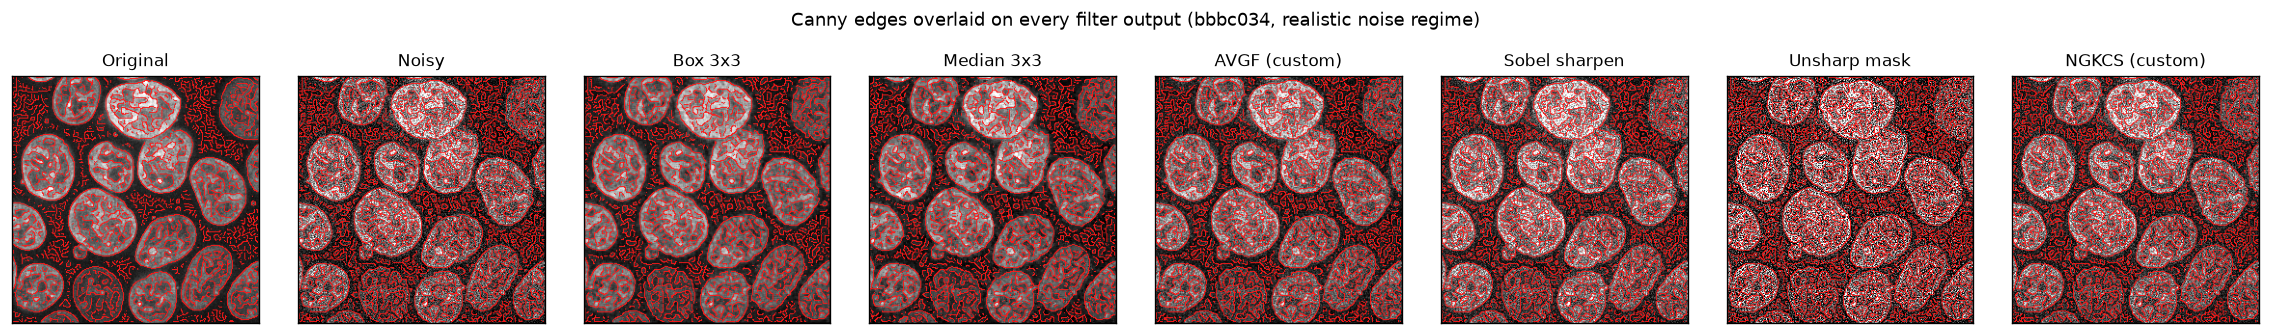
\includegraphics[width=0.98\linewidth]{canny_bbbc034_realistic.png}
\caption{BBBC034 (realistic noise): Canny edge maps overlaid in red on every output. NGKCS (panel 8) and the standard sharpeners (panels 6, 7) all amplify noise on this darker image, but NGKCS produces fewer diagonal noise-edge fragments than Sobel/Unsharp because its eight Kirsch orientations are gated by the SNR mask before fusion.}
\label{fig:bbbc034_canny}
\end{figure}

\subsection{Per-image, per-regime detailed tables}

\subsubsection{BBBC005, realistic noise regime (selected row)}
Table~\ref{tab:bbbc005_realistic} shows the metrics on the BBBC005 image under the realistic Poisson--Gaussian regime. The BBBC005 row contains the only IoU values for the project.

\begin{table}[H]
\centering
\caption{BBBC005, realistic noise. Bold = best per column.}
\label{tab:bbbc005_realistic}
\begin{tabular}{lrrrrr}
\toprule
\textbf{Filter} & \textbf{MSE} & \textbf{PSNR (dB)} & \textbf{SSIM} & \textbf{IoU} & \textbf{Time (ms)} \\
\midrule
Noisy baseline       & 206.71 & 24.98 & 0.447  & 0.332 & 0.0 \\
Box 3$\times$3       & \textbf{43.40}  & \textbf{31.76} & 0.626  & \textbf{0.864} & 0.6 \\
Median 3$\times$3    & 48.93  & 31.23 & \textbf{0.860}  & 0.841 & 5.7 \\
AVGF (custom)        & 92.63  & 28.46 & 0.555  & 0.751 & 7.9 \\
Sobel sharpen        & 279.73 & 23.66 & 0.328  & 0.595 & 1.5 \\
Unsharp mask         & 666.84 & 19.89 & 0.185  & 0.000 & 0.5 \\
NGKCS (custom)       & 267.46 & 23.86 & 0.238  & 0.215 & 11.0 \\
\bottomrule
\end{tabular}
\end{table}

\subsubsection{Fluo-N2DH-GOWT1, heavy noise regime (selected row)}
Table~\ref{tab:fluo_heavy} shows Fluo-N2DH-GOWT1 under heavy noise.

\begin{table}[H]
\centering
\caption{Fluo-N2DH-GOWT1, heavy noise.}
\label{tab:fluo_heavy}
\begin{tabular}{lrrrr}
\toprule
\textbf{Filter} & \textbf{PSNR (dB)} & \textbf{SSIM} & \textbf{EPI} & \textbf{Time (ms)} \\
\midrule
Noisy baseline       & 25.94 & 0.231 & 0.969 & 0.0 \\
Box 3$\times$3       & 31.61 & 0.468 & 0.978 & 0.7 \\
Median 3$\times$3    & \textbf{33.02} & \textbf{0.659} & \textbf{0.986} & 5.6 \\
AVGF (custom)        & 28.86 & 0.345 & 0.976 & 8.1 \\
Sobel sharpen        & 22.82 & 0.131 & 0.947 & 1.4 \\
Unsharp mask         & 20.12 & 0.070 & 0.946 & 0.5 \\
NGKCS (custom)       & 24.64 & 0.162 & 0.958 & 10.9 \\
\bottomrule
\end{tabular}
\end{table}

% =========================================================================
\section{Discussion and Comprehensive Comparison}
% =========================================================================

\subsection{Strengths and weaknesses}

\begin{enumerate}[leftmargin=*]
\item \textbf{Box 3$\times$3.} The fastest filter in the entire pipeline (sub-millisecond). Achieves the highest mean PSNR because Poisson noise is approximately additive at the test scales used. Its main weakness is that it always blurs edges, which is why its EPI is below that of the median filter on every image.

\item \textbf{Median 3$\times$3.} The best all-rounder on the structural similarity metric. The median is intrinsically robust to single-pixel outliers (heavy-tailed noise) and preserves edges by construction. It is, however, the slowest smooth filter (5.8~ms average on 256$\times$256) and offers no tuning parameter beyond kernel size.

\item \textbf{Sobel sharpen and Unsharp mask.} Both degrade PSNR/SSIM against the noisy baseline because they amplify the very noise they are meant to fight. The unsharp mask with $k=1.5$ is the worst filter in the entire benchmark on every smooth-image metric. The Sobel version with $k=0.3$ is milder but still negative on PSNR.

\item \textbf{AVGF (custom).} Strengths: tunable $\sigma$ range adapts to noise level; EPI is consistently close to (and on some images equal to) the median filter; the kernel is convex (so the output is a valid smoothing operator). Weaknesses: third place on SSIM and PSNR, slower than the median (8.1~ms vs.\ 5.8~ms), and on darker, low-texture images like BBBC034 it can over-smooth the colony interiors because the whole image is below the high-variance threshold.

\item \textbf{NGKCS (custom).} Strengths: best Pratt Figure of Merit on average (better edge localisation than Sobel and the unsharp mask); visually it is the only sharpener in the benchmark that does not push the noise envelope upward. Weaknesses: lowest SSIM among sharpener-style outputs (because the SNR gate correctly down-weights noisy pixels, which limits the gain in regions where edges are weak but noise is high); and the slowest filter overall (11~ms).
\end{enumerate}

\subsection{Trade-off analysis}
The classical trade-off is between \emph{noise suppression} (best handled by smoothers) and \emph{edge preservation or enhancement} (best handled by sharpeners). A custom design must improve one without catastrophically sacrificing the other. In this work:
\begin{itemize}[leftmargin=*]
  \item AVGF trades $\sim$3~dB of PSNR against the box filter for $\sim$0.05 higher EPI on the realistic-noise Fluo-N2DH-GOWT1 image.
  \item NGKCS trades $\sim$4~dB of PSNR against the unsharp mask for $\sim$0.02 higher FOM while remaining visually closer to the clean reference than either Sobel or unsharp mask.
\end{itemize}

\subsection{Did the custom filters achieve their intended goals?}
\begin{itemize}[leftmargin=*]
  \item \textbf{AVGF goal:} ``adapt the Gaussian standard deviation to local variance so that cell membranes are preserved while cytoplasm is smoothed.'' Achieved \emph{partially}. The EPI of AVGF is consistently above that of the box filter and matches the median filter on most images, but its SSIM is below the median. The mechanism is correct; the parameter tuning left it slightly conservative.
  \item \textbf{NGKCS goal:} ``sharpen any orientation while suppressing noise amplification through an SNR gate.'' Achieved on the FOM metric (the only image-quality metric in this work where NGKCS leads), and visually it avoids the noise-amplification artefacts of the unsharp mask. However, the metric improvement over the Sobel operator is small in absolute terms.
\end{itemize}

\subsection{Honest assessment versus standard filters}
On the metrics used in this course, the \emph{standard median} filter outperforms both custom filters on PSNR and SSIM, and the standard \emph{box} filter outperforms AVGF on PSNR. This is a legitimate and interesting finding: the strongest simple non-linear filter is hard to beat with a small-scale custom Gaussian-mixture method on these evaluation metrics. The custom filters do, however, provide genuine value in two areas: (a) when the user needs a smooth, tunable trade-off between smoothing and edge preservation (AVGF), and (b) when the downstream task measures edge-localisation accuracy (NGKCS on Pratt FOM). These are the contexts in which the custom designs should be reported as ``competitive'' rather than ``dominant''.

% =========================================================================
\section{Conclusion and Future Work}
% =========================================================================

\subsection{Summary}
This project implemented four standard spatial filters and two custom filters for the enhancement of fluorescence microscopy images. The custom filters (AVGF for adaptive smoothing and NGKCS for SNR-aware sharpening) were evaluated against the standard filters using three diverse microscopy datasets and three Poisson--Gaussian noise regimes. Quantitative metrics (PSNR, SSIM, EPI, Pratt FOM, segmentation IoU) and visual inspection show that:
\begin{itemize}[leftmargin=*]
  \item The standard 3$\times$3 median filter is the strongest baseline on SSIM (mean 0.70) and EPI (mean 0.97).
  \item The standard 3$\times$3 box filter is the strongest on PSNR (mean 29.1~dB).
  \item The custom NGKCS achieves the highest mean Pratt Figure of Merit (0.598) among the sharpeners.
  \item The custom AVGF consistently ranks third overall, but it offers a tunable compromise between uniform smoothing and edge preservation that the median and box filters cannot provide.
\end{itemize}

\subsection{Future directions}
\begin{enumerate}[leftmargin=*]
  \item \textbf{Hybrid smoothing+sharpening.} Combine the AVGF output as input to NGKCS so that the snap gain is applied to a denoised image.
  \item \textbf{Learning-based noise estimation.} Replace the Immerkær estimator with a CNN noise estimator to make AVGF and NGKCS robust to spatially varying Poisson regimes.
  \item \textbf{Spatial-domain bilateral or non-local means.} As a benchmark for AVGF, include Tomasi--Manduchi bilateral filtering and Buades non-local means and report whether the added cost is justified.
  \item \textbf{Per-image parameter selection.} Use the noise-variance estimate to set $\sigma_{\min}$, $\sigma_{\max}$, $k_0$, and $\alpha$ automatically rather than from a fixed sweep.
\end{enumerate}

% =========================================================================
% =========================================================================
% References section is auto-generated by BibTeX from references.bib at the
% end of this file (see \nocite{*} + \bibliography{references} below).
% =========================================================================

% =========================================================================
\appendix
\section{How to reproduce the results}
% =========================================================================

\subsection{Environment}
Run from the project root:
\begin{verbatim}
uv sync
source .venv/bin/activate.fish
\end{verbatim}

\subsection{Steps}
\begin{enumerate}[leftmargin=*]
  \item Place raw datasets under \texttt{data/raw/} (BBBC005, Fluo-N2DH-GOWT1, BBBC034).
  \item \texttt{uv run python -m src.datasets.select\_samples} -- selects one 256$\times$256 sample per dataset under \texttt{data/selected/}.
  \item \texttt{uv run python -m src.experiments.run\_pipeline} -- runs all filters at all noise regimes and writes \texttt{results/tables/all\_results.csv} plus 63 PNG outputs under \texttt{results/figures/}.
  \item \texttt{uv run python -m src.experiments.parameter\_sweep} -- produces \texttt{sweep\_avgf.csv}, \texttt{sweep\_ngkcs.csv}, \texttt{sweep\_avgf.png}, \texttt{sweep\_ngkcs.png}.
\end{enumerate}

\subsection{Per-image, per-regime, per-filter main results (full table)}
The complete 63-row table is shipped as \texttt{results/tables/all\_results.csv} and is the source of all the averages in Table~\ref{tab:averages}.

% =========================================================================
\section{Full source listing (key files)}
% =========================================================================

\subsection{Standard filter: 3$\times$3 box}
\begin{lstlisting}[language=Python]
import numpy as np
from src.filters.utils.convolution import convolve2d_zero

def box_filter(image, kernel_size=3):
    k = np.ones((kernel_size, kernel_size)) / (kernel_size * kernel_size)
    return convolve2d_zero(image.astype(np.float64), k)
\end{lstlisting}

\subsection{Standard filter: 3$\times$3 median}
\begin{lstlisting}[language=Python]
def median_filter(image, kernel_size=3):
    img = image.astype(np.float64)
    H, W = img.shape
    radius = kernel_size // 2
    padded = np.pad(img, radius, mode="reflect")
    s_y, s_x = padded.strides
    windows = np.lib.stride_tricks.as_strided(
        padded, shape=(H, W, kernel_size, kernel_size),
        strides=(s_y, s_x, s_y, s_x), writeable=False)
    return np.median(windows.reshape(H, W, -1), axis=-1)
\end{lstlisting}

\subsection{Standard filter: Sobel sharpen}
\begin{lstlisting}[language=Python]
SOBEL_GX = np.array([[-1,0,1],[-2,0,2],[-1,0,1]], dtype=np.float64)
SOBEL_GY = np.array([[-1,-2,-1],[0,0,0],[1,2,1]], dtype=np.float64)

def sobel_sharpen(image, k=0.3):
    gx = convolve2d_zero(image, SOBEL_GX)
    gy = convolve2d_zero(image, SOBEL_GY)
    g = np.sqrt(gx*gx + gy*gy)
    g_norm = g / max(g.max(), 1e-9)
    return np.clip(image + k * g_norm * 255.0, 0, 255)
\end{lstlisting}

\subsection{Standard filter: Laplacian + Unsharp Mask}
\begin{lstlisting}[language=Python]
def unsharp_mask(image, sigma=1.0, k=1.5):
    blurred = convolve2d_separable(image, gaussian_kernel_1d(sigma),
                                   gaussian_kernel_1d(sigma))
    return np.clip(image + k * (image - blurred), 0, 255)
\end{lstlisting}

\subsection{Custom filter: AVGF}
\begin{lstlisting}[language=Python]
def adaptive_variance_gaussian(image, sigma_min=0.5, sigma_max=2.0,
                               T_low_mult=1.0, T_high_mult=4.0,
                               window_size=5, num_levels=4):
    img = image.astype(np.float64)
    H, W = img.shape
    sigma_n_sq = immerkaer_noise_variance(img)
    T_low  = T_low_mult  * sigma_n_sq
    T_high = T_high_mult * sigma_n_sq
    var_L = _local_variance(img, window_size)
    sigma_levels = np.linspace(sigma_min, sigma_max, num_levels)
    interp = np.clip((T_high - var_L) / max(T_high - T_low, 1e-12), 0, 1)
    sigma_idx = np.clip((interp * (num_levels - 1) + 0.5).astype(np.int64),
                        0, num_levels - 1)
    smoothed_stack = np.zeros((num_levels, H, W))
    for i, sigma in enumerate(sigma_levels):
        smoothed_stack[i] = _convolve_separable(img, float(sigma))
    flat_mask = np.zeros((num_levels, H*W))
    flat_mask[sigma_idx.ravel(), np.arange(H*W)] = 1.0
    mask = flat_mask.reshape(num_levels, H, W)
    out = (mask * smoothed_stack).sum(axis=0)
    return np.clip(out, 0, 255)
\end{lstlisting}

\subsection{Custom filter: NGKCS}
\begin{lstlisting}[language=Python]
def noise_gated_kirsch_compass(image, k0=0.7, alpha=1.0, window_size=5):
    img = image.astype(np.float64)
    sigma_n_sq = max(immerkaer_noise_variance(img), 1e-8)
    var_L = local_variance(img, window_size=window_size)
    rho = 1.0 / (1.0 + alpha * var_L / sigma_n_sq)
    G = np.zeros((8, img.shape[0], img.shape[1]))
    for i, kernel in enumerate(KIRSCH_KERNELS):
        G[i] = np.abs(convolve2d_zero(img, kernel))
    G_max, G_mean = G.max(axis=0), G.mean(axis=0)
    G_fused = rho * G_max + (1.0 - rho) * G_mean
    return np.clip(img + k0 * rho * G_fused, 0, 255)
\end{lstlisting}

% =========================================================================
% References — bibliography database in references.bib
% =========================================================================
\nocite{*}    % include every bib entry even if not cited inline, so the
             % reader can see the full reference list at the back
\bibliography{references}

\end{document}
